% !TeX root =thesis.tex

\chapter{Introduction}
%Superfluidity in many-body fermionic system is one of the most dramatic and fascinating topic in physics. It calls the attention and effort from generation of physicists.  The study is dominated with one particular fermions, electrons.  However, this system suffers from one difficulty as the interaction  in a particular system is usually fixed and cannot be tuned experimentally.  
From  a methodological view, a physics system  would be very desirable for developing and  verifying a theory for it if  it can be described with  as few parameters as possible and  each parameter  is as tunable as possible. One of such systems is dilute fermionic alkali gas with Feshbach resonance.  Dilute fermionic alkali gas was cooled into degenerate region in 1999 \cite{DeMarco1999}; not long afterward,  superfluidity was observed for such systems in 2003 \cite{Regal2003}.  In dilute ultracold fermionic alkali gas, it is sufficient in many analyses to describe an atom-atom interaction with one single parameter, s-wave scattering length, $a_{s}$, because the gas is dilute and experiments are carried out at very low temperature.       

The other desirable property is the ability to  tune the effective interaction strength, or s-wave scattering length, $a_{s}$ through the Feshbach resonance.  One energy level of an atom  usually splits into several hyperfine levels in a magnetic field  due to the hyperfine interaction between nuclear spin and electronic spin. Hyperfine spin indices provide a good set of quantum numbers for a single atom.  In the theory of  atom-atom interactions, a channel refers to a  configuration of hyperfine spin indices of one atom-atom pair. In the magnetic field, different channels often have different Zeeman energies, which can be tuned by the magnetic field.  In addition, a channel is no longer an eigenstate for the atom-atom interaction because it is mostly due to the overlap between two atoms' electrons.  In other words, different channels are hybridized.  The potential of each channel is also different.  The potential of one  channel (closed-channel) may be deep enough to sustain a bound state.  In a certain magnetic field,  this bound state level might be close to the zero-energy threshold of the other channel (open-channel) and  dramatically modify the low-energy scattering property in that channel.   In such a situation, two atoms approaching each other in the open-channel may spend certain amount of time in the closed-channel and then reemerge in the open-channel.  Atoms in the open-channel seem to feel an enhanced effective interaction.  This phenomenon is known as Feshbach resonance.    We will get to more quantitative analysis about alkali gas in Chpater \ref{sec:intro:one} and Feshbach resonance in two-body context in Chapter \ref{sec:intro:twobody}. 




A very desirable property of the Feshbach resonance is that the effective interaction is tunable experimentally because the Zeeman energy difference is tunable though  instruments such as a magnetic field.  
This unique ability gives physicists a rare opportunity to study  a many-body system under various interaction strength, which connects different physics originally developed separately.  Particularly for the fermion system, there are a series of  theoretical works about uniform treatment over BEC and BCS since the 1960s \cite{Eagle,LeggettCrossover,Nozieres,RanderiaBEC}, for which dilute ultracold alkali gas with the Feshbach resonance provides the perfect testing grounds.  Indeed,  the theory works quite well  qualitatively.  

%One important characteristic quantity of Feshbach resonance is $\delta_{C}$N (see detail in Chapter \ref{sec:intro:twobody} for details): when detuning from resonance is smaller than it, open-channel atoms dominate and closed-channel can be neglected.  The effective interaction can still be characterized by $a_{s}$.  One seems to acquire a ``magic knob'' that can tune the interaction between atoms.  On the other hand, when negative tuning is much larger than $\delta_{C}$, atoms in closed-channel have comparable weight to that of open-channel or even dominate them.  Two channels need to be considered at the same time.  


%This thesis tries to look into the idiosyncrasy of the Feshbach resonance in contrast with a true ``Simple'' knob of the interaction strength.
\begin{figure}[htbp]
\begin{center}
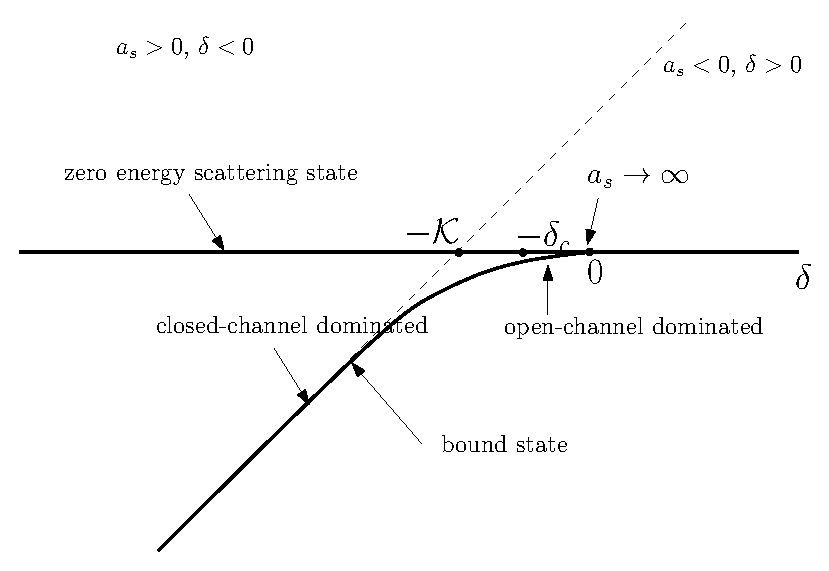
\includegraphics[width=0.8\textwidth]{levels}
\caption{Energy levels in the Feshbach resonance\label{fig:intro:levels}} 
\parbox{0.7\textwidth}{\small $\delta$ is the detuning from the resonance point.  The horizontal line stands for the zero energy scattering state, $\psi\sim\nth{r}-\nth{a_s}$, which exists for any detuning.  The lower line stands for the bound state, which only exists for negative detuning ($\delta<0$, $a_s>0$). The dash line stands for the closed-channel bound state.  An interesting point to see is that the bound state appears earlier than the cross point of the closed-channel bound state level and zero energy. When the detuning is smaller than $\delta_c$, this real bound state is composed most with atoms in the open-channel. See Chapter \ref{sec:intro:twobody} for details.   }

\end{center}
\end{figure}

  The two-body theory of Feshbach resonance has a characteristic  parameter, $\delta_c$ (see Fig. \ref{fig:intro:levels}).  Na\"{i}vely speaking, in the negative detuning side of any resonance, particles should mostly stay  in a (virtual) bound-state of closed-channel (or similar) resonances.  However, at the resonance point  of Feshbach resonance, atoms is mostly in the open-channel, and it does so up to a negative detuning of $\delta_c$. Only when the detuning from resonance is much larger than $\delta_c$, atoms have the majority weight in the closed-channel.    Moving to a many-body problem, an important question is how this energy scale compares to a typical many-body energy scale, the Fermi energy. In the region not too far away from resonance ($\delta\ll\delta_{c}$), the closed-channel weight is negligible, if the Fermi energy is much smaller than $\delta_c$, (i.e., \emph{broad resonance}).  Crossover experiments usually perform at detuning not too far away from the resonance, where the closed-channel can be safely ignored at many-body level. Eventually, when the detuning is negatively enough, $\delta\gg\delta_{c}$, the bound state is almost like the closed-channel bound state with small dressing from the open-channel.  We nevertheless do not concern such cases in the broad resonance because crossover phenomena are well covered in both (BEC and BCS) ends with $\delta\ll\delta_{c}$. The problem can be well-described as a two-species fermion system with a tunable interaction.  The Feshbach resonance indeed serves as a simple ``magic'' knob for the interaction strength.  The original  theories developed on  single-channel models  apply to this case directly.  This is also the situation for the popular experiment systems (${}^{6}\text{Li}$ at 834G, $^{40}\text{K}$ at 224G).   Many theoretical works are developed over those original works along such simple single-channel models. On the contrary, when the Fermi energy is  comparable to or even larger than $\delta_c$, the closed-channel has to be included in the many-body level even for small detuning from the resonance. Such situation was considered in  theoretical works such as \cite{GurarieNarrow} and is the focus of the current thesis. 
  
  Nevertheless, one crucial simplification comes from  the assumption that closed-channel bound state is relatively tight bound, and is much smaller than  many-body scales, such as interparticle distance, (but often larger than potential range).  Therefore, it is not necessary to handle all the  fermion species simultaneously, which probably requires quite different techniques to solve. Instead, two channels can still be treated successively. 
x
To complicate the problem even further,  real experiment setups often have one common hyperfine species between two channels. There are three hyperfine species in two channels instead of four species (two for each channel).  Two most popular setups (${}^{6}\text{Li}$ at 834G, $^{40}\text{K}$ at 224G) are both three-species ones although they are the broad resonance.  Pauli exclusion prevents  both channels from occupying the same level simultaneously because of this common species.  This peculiar effect has no counterpart in two-body physics. It has  received little theoretical attention.    Some  narrow resonances do exist \cite{ChinRMP} and it is not totally inconceivable to conduct many-body experiments with those resonances.  The central concern in this thesis is about such situations. 

Roughly speaking, becoming many-body brings three effects to the original two-body problem.  The first one closely associates with the Fermi energy.  At low temperature, most fermions are inactive and only fermions close to the Fermi surface participate in various interaction. Therefore, energy often needs to be measured from the Fermi surface instead of zero as in the two-body situation.  This effect has been extensively studied in \cite{GurarieNarrow}.

The second effect is about counting. Unlike the single-channel problem, there are two densities in the two-channel problem, the density of atoms in open-channel, $n_{o}$, and the density of atoms in closed-channel, $n_{c}$. When the closed-channel weight is small (broad resonance), it is all right to treat the total density as the same as the open-channel density.  However, in the narrow resonance, where the closed-channel weight is not negligible, counting becomes complicated.  Extra care is required to specify which channel the  quantities, such as ``density'', belong.  This effect has been  also extensively studied in \cite{GurarieNarrow}.

The last effect is unique for the three-species problem, where one common species is shared by both channels.  The phase spaces of two channels are overlapped because of the Pauli exclusion caused by the common species. This effect is controlled by the overlapping of states in two channels. A rough estimate can be made.  The closed-channel bound-state which is in resonance with the open-channel zero energy threshold is relatively small.  Its binding energy $E_b$ is close to absolute Zeeman energy difference between two channels, $\eta$.  On the other hand, fermions in the open-channel fill the lowest  momentum state up to typically the Fermi energy, $E_F$.  Therefore ratio $E_F/\eta$ is expected to control the overlapping effect. This effect is not addressed in any theoretical work to this author's knowledge.  How it modifies the many-body picture is the center topic of this thesis. 

Alternatively, we can make a rough estimate using two-fermion molecule gas. We assume the molecule size is $a_{c}$ and the total number is $N$.  Assuming further that the bound-state is close to threshold,   the bound-state wave function can then be written as $A/(k^{2}+\kappa^{2})$, where $\hbar^{2}\kappa^{2}/2m=E_{b}$, (see Appendix \ref{sec:pathInt2:short-range}). ``$A$'' can be obtained by normalization, $\sum_{k=0}^{1/a_{c}}\abs{\psi}^{2}\sim{}N$. Now  we consider only particles in the typical many-body scale, i.e. the Fermi energy, $E_{F}$, which is going to overlap with levels occupied in the open-channel. The Fermi energy is much smaller than the energy scale of the closed-channel bound state, $E_{F}\ll\kappa$.  The total particle in this range is roughly $N\cdot(k_{F}a_{c})^{3}$, which is much smaller than $N$. Put this into the perspective of the two-channel problem, the low momentum,  ($k\lesssim{}k_F$), is still dominated by the open-channel component even when the total number of atoms in the closed-channel is comparable or higher than the total number  of atoms in the open-channel because atoms in the closed-channel are mostly in the high-momentum states.     

 We review several important concepts in Chapter \ref{sec:intro:one} to Chapter \ref{sec:intro:1channel}. And then we present my main work in Chapter \ref{ch:path2} and an earlier attempt using a roughly equivalent but less-flexible approach in Appendix \ref{ch:mean}.  Chapter \ref{sec:intro:one} briefly reviews  dilute ultracold alkali gas.   Particularly, section \ref{sec:intro:as} examines the idea of ``universality'', which is one of the central ideas in our treatment of the two-channel model.  Chapter \ref{sec:intro:twobody} goes over the Feshbach resonance in two-body physics, where the concept of  the narrow (broad) resonance is introduced. Chapter \ref{sec:intro:1channel} reviews the single-channel BEC-BCS crossover problem as well as the path-integral approach to solve it, which serves as the starting point of the two-channel model. After these reviews, we present our work about the narrow Feshbach resonance within a many-body path-integral framework in  Chapter \ref{ch:path2}.   Appendix \ref{ch:mean} includes our earlier attempt   using BCS ansatz  approach in mean-field level.  Chapter \ref{ch:conclusion} discusses and concludes our approach.  

\chapter{Dilute ultracold alkali gas}\label{sec:intro:one}
Dilute ultracold alkali gas became experimentally realized since the 1990s.  Not long after the bosonic ones, fermionic Alkali gas was also available in degenerate region.  Because of the ultra-low temperature (in the order of nK), and diluteness ($10^{12}\sim10^{15}\text{cm}^{-3}$), the system is mostly \emph{free} except when atoms are close.   This particular properties simplifies the theoretical analysis tremendously (see Sec. \ref{sec:intro:as} for detail).  In this section, we covers a few aspects that closely related to the current thesis.     

\section{A single atom and hyperfine levels}
In experiments of ultracold alkali gas, magnetic field ($\mathbf{B}$) is the most common physical quantity to manipulate.  First we study a  single isolated atom.  For an alkali atom, there is only one electron in the outer shell, and rest electrons are in the filled inner shells, which have no total magnetic moment.  So only the outermost electron interact with magnetic field through electronic spin, $\mathbf{S}$.  Furthermore, magnetic field also interacts with nuclear spin, $\mathbf{I}$.  The full spin-part Hamiltonian is
\begin{equation}
\begin{split}\label{eq:intro:1atom}
H_{spin}&=A \mathbf{I}\cdot\mathbf{S}-\mu_{e}\mathbf{B}\cdot\mathbf{S}-{\mu}_{n}\mathbf{B}\cdot\mathbf{I}\\
&=A \mathbf{I}\cdot\mathbf{S}-\mu_{e}{B}{S_{z}}-{\mu}_{n}{B}{I_{z}}
\end{split}
\end{equation}
The first term in both lines describes the hyperfine interaction, while the next two terms describe Zeeman energy of electrons and nuclei respectively. $\mu_{e}$ is electron magnetic moment, and $\mu_n$ is the nuclear magnetic moment.  In the second line, we take the direction of magnetic field as z-direction. This Hamiltonian can be diagonalized with the help of total spin 
\begin{equation}
\mathbf{F}=\mathbf{S}+\mathbf{I}
\end{equation}
When the magnetic field is zero, $(F,F_{z})$ are good quantum numbers. Furthermore, all states with the same total spin $F$ are degenerated.   When the magnetic field is finite, $(F,F_{z})$ are no longer good quantum numbers. Nevertheless, we can still label states with these two numbers via their adiabatic connection to zero magnetic field.  For a finite magnetic field, besides states with the highest and lowest $F_{z}=\pm{}F$, each state is a mix of different $(S_{z}, I_{z})$ or $(F,F_z)$.  Fortunately, $S=1/2$ for alkali gas,  so each state is mixed with maximum of two sets $(S_{z}, I_{z})$. At a high magnetic field, the first hyperfine coupling term in Eq. \eqref{eq:intro:1atom} is dominated by the last two terms and  eigenstates are approximately described by quantum numbers $(S_{z},I_{z})$.  (Please refer to Fig. \ref{fig:intro:li6}.)

\begin{figure}[htbp]
\begin{center}
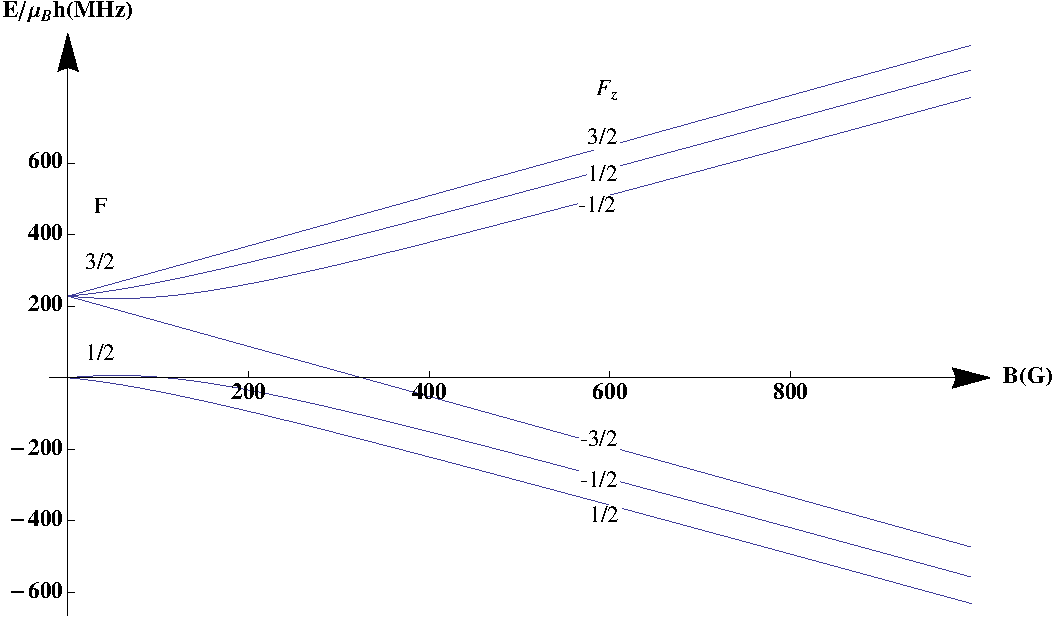
\includegraphics[width=0.8\textwidth]{hyperfineLi6}
\caption{Hyperfine structure of a single \textsuperscript{6}Li atom } 
Levels are marked with $F$ and $F_{z}$ {(see Footnote \ref{foot:intro:f} in page \pageref{foot:intro:f})}
\label{fig:intro:li6}
\end{center}
\end{figure}



\section{Two-body interactions}
Things would be very boring if there was only the single-atom Hamiltonian.  Before we discuss the interaction itself, we introduce one important concept related.   The basic unit with interaction is a pair of atoms.  A ``channel'' is used to refer one  configuration of hyperfine spins for a pair, $\ket{F^{(1)},F_{z}^{(1)}}\otimes\ket{F^{(2)},F_{z}^{(2)}}$  \footnote{Remember that $(F,F_{z})$ are only labels, and do not stand for the total angular momentum unless no magnetic field.\label{foot:intro:f}}    Channels are good basis for non-interaction pair.  A pair of atoms in one channel would stay in it forever if no interaction between them.  Now let us get back to alkali atoms.  Two alkali atoms interact mostly through the overlapping of their electron clouds in the dilute setup.  Thus besides the atom-atom distance, the interaction is mostly a function of electronic spins only, with little-to-none dependence on nuclear spins.  Schematically the interaction can be written as 
\begin{equation}\label{eq:intro:two}
V=f(r)+g(r)\mathbf{S_{1}}\cdot\mathbf{S_{2}}
\end{equation}
The hyperfine levels that diagonalize the single atom Hamiltonian is no longer eigenstates for this interaction.  In another word, the interaction has non-diagonal terms over channels and therefore hybridizes them. Instead, states with definite electronic spins form a good basis for the two-atom interaction.  Nonetheless, most experiments are performed in the so-called high-field region where the electronic spin $S_z$ is approximately a good quantum number, and therefore the original hyperfine levels (channels) serve as a good starting point as the zeroth order.  When the hybridization is considered, multichannel scattering is possible.  The most interesting thing in the multi-channel scattering is resonance.  One of them is Feshbach resonance.  Potential in one channel may be deep enough to sustain a bound-state. When this bound-state energy is close to the zero-energy threshold in the other channel, low-energy scattering properties in that channel is dramatically modified.  This resonance turns out to be extremely useful in   cold atom experiments.  Chapter \ref{sec:intro:twobody} reviews its theory in  two-body physics; the more involving many-body problem is then the central theme of this thesis. 

Let us discuss one example.  In popular experiments setup for $^{6}$Li (Fig. \ref{fig:intro:li6}), usually experiments are prepared with atoms in the two lowest hyperfine levels, described by the  direct product, $\ket{F=\nth{2},F_{z}=-\nth{2}}\otimes\ket{F=\nth{2},F_{z}=+\nth{2}}$.  This is a good approximation until when two atoms are very close.  Recall that the two-atom interaction (Eq. \ref{eq:intro:two}) conserves the z-component of total angular momentum, $F_{z}^{(1)}+F_{z}^{(2)}$.  Therefore this states mixed with four other possible channels, $\ket{\nth{2},-\nth{2}}\otimes\ket{\frac{3}{2},+\nth{2}}$, $\ket{\frac{3}{2},-\nth{2}}\otimes\ket{\nth{2},+\nth{2}}$, $\ket{\frac{3}{2},+\frac{3}{2}}\otimes\ket{\frac{3}{2},-\frac{3}{2}}$, $\ket{\frac{3}{2},+\frac{1}{2}}\otimes\ket{\frac{3}{2},-\frac{1}{2}}$ (All states is labeled as $\ket{F,F_{z}}$).  There are plenty of chances for resonance, and indeed, there are several of them.  Note that close to the resonance, it is normally sufficient to consider only the  channel that is in resonance, while neglect all others.  Another important aspect is whether the two channels share one single hyperfine species (three species in total) or not (four species in total).   The closed channel in the most studied resonance close 834G is approximately $\ket{\frac{3}{2},-\nth{2}}\otimes\ket{\nth{2},+\nth{2}}$ and the resonance is a three-species one\cite{ZhangThesis,ChinRMP}. 

\section{Universality,  the Bethe-Peierls boundary condition, the s-wave scattering length, the two-body density matrix\label{sec:intro:as}}
One important aspect of the interaction in dilute ultracold alkali gas is that for many purposes, it is sufficient to characterize the interaction  by a single two-body parameter, the s-wave scattering length, $a_s$,  because  both the density and the temperature are so low.  Often this is  interpreted as we can replace the real potential with a pseudo potential, $U(\vr)=\frac{4\pi{}a_{s}\hbar^{2}}{m}\delta(\vr)$\cite{pethick, LeggettBEC}.  Nevertheless, an alternative interpretation about $a_s$ is more useful in this work\cite{LeggettBEC, Tan2008-1,Tan2008-2,CombescotTan}.  For the short-range potential, where the potential range, $r_c$, is much smaller than the average interparticle distance, $a_0$, it is not hard to see that in the majority of the time, particles are free-like.  They only interact  when two particles are close to each other.  We can schematically divide the full space into two domains: $\mathcal{D}$, where any two particles are more than $a_c$ away from each other; and otherwise, $\mathcal{I}$. Most physical quantities would be very easy to calculate if only considering the free part, $\mathcal{D}$.  This is almost true in the dilute gas, with modification on a special  boundary condition.  The effect of the potential on wave-function in the short-range region, $\mathcal{I}$, is to enforce the boundary condition on the free part $\mathcal{D}$, $\psi(r)\xrightarrow{r\to0}\psi_{0}(r)$.  For an isometric $\psi_{0}(r)$, the lowest order in radial coordinator $r$ is $\nth{r}$.   Including the next order, a constant,  we have $\psi_{0}(r)=\nth{r}(1-\frac{r}{a_{s}})$ barring the normalization.  All these consideration gives us the simplest non-trivial boundary condition on the radial component of a wave function
\begin{equation}\label{eq:intro:Bethe}
\psi(r)\xrightarrow{r\to0}A\br{\nth{r}-\nth{a_s}}
\end{equation}
which is also known as Bethe-Peierls boundary condition\cite{BethePeierls}.  We neglect all the three-body or more-body interaction, which is a reasonable assumption for the dilute gas. Therefore,  $a_{s}$ is completely determined by two-body physics.  And   this simple boundary condition applies to two-body, few-body, as well as many-body systems, and proves to be a very powerful tool to various problems.  

Eq. \ref{eq:intro:Bethe} coincides the zero-energy s-wave scattering wave function, which explains the name of parameter ``$a_s$'', s-wave scattering length. Nevertheless,   note we did not mention anything about zero energy, where $a_{s}$ is defined in the scattering theory context.  In fact,  this boundary condition applies generally to  any low (positive or negative) energy solutions as long as the energy involved is much lower than the energy scale in the interaction domain $\mathcal{I}$.  Hence this boundary condition can be easily  applied  to close-to-threshold bound state as well.  The s-wave wave function of a weak bound-state is $\psi(r)=\nth{r}e^{-r/a_s}$ in $\mathcal{D}$,\footnote{The extra $\nth{r}$ factor is there for  radial wave function in 3D.} which matches the Bethe-Peierls boundary condition with a positive $a_{s}$ (for  $r\ll{}a_{s}$), and we have the often cited relation for binding energy $E_{b}$.
\begin{equation}
 E_{b}=\frac{\hbar^{2}}{2m_{r}a_{s}^{2}}
\end{equation}
Here $m_{r}$ is the reduced mass for center of mass, which is equal to half of the atom mass for a pair of the same atoms.  This immediately clears one often confusing and counter-intuitive fact, that a positive  $a_s$ corresponds to the bound state.  If interpreting in the normal scattering theory, a positive $a_s$  usually associates with a repulsive interaction, which obviously does not support a bound state.\footnote{This seemingly paradox can be resolved carefully within scattering theory as following. In scattering theory, the fact that  repulsive interaction leads to positive phase shift and therefore positive $a_s$, and attractive interaction leads to negative phase shift and negative $a_s$, is only true when interaction is weak, and phase shift as well as $a_s$ is small.  At the strong interaction, where a bound state is formed, phase shift changes $2\pi$; $a_s$ is large and  changes sign over the threshold. The positive or negative relationship does no longer hold.}

 The s-wave scattering length, $a_s$, or Eq. \ref{eq:intro:Bethe}, does not fix the normalization on the wave function. This normalization factor, encapsulating many-body effects, shows up in many physical quantities.  In a dilute and low-energy system,  its square is proportional to  \emph{integrated contact intensity}, $C$, defined in \cite{ Tan2008-1,Tan2008-2,CombescotTan}, besides a simple constant factor and total density.  At the limit where $a_c\to0$, $C$ and $a_s$ alone, can describe several important physical quantities, (for example internal energy).  A particular useful one for this thesis is the limit at high-momentum distribution of particles, 
 \begin{equation}
 n_k=\frac{C}{k^4}
 \end{equation}
 Note that here \emph{high-momentum} does not mean the absolutely high-momentum, it means lower than the characteristic momentum of potential $1/r_c$, but higher than any other scale, $1/a_0$,...  
 Indeed, when the short-range approximation and low-energy approximation apply, we expect that two-body correlation at  high-momentum ($\gg{k_{F}}$) does not change much from a two-body system to a many-body system.  In this high-energy region, we can always use   the two-body wave function as good approximation. 
 
 In many-body physics, lots of physical observable quantities relate to one set of  quantities, density matrix, $\av{\Psi^\dg\Psi^\dg\cdots\Psi\Psi}$. In fermionic system,  one-body density matrix is often very close to the free case, although the difference can be important for various theories (such as Landau Fermi liquid theory).  A two-body density matrix is often  used for phenomena with  more qualitative difference, such as pairing. Formally, we can decompose a two-body density matrix into orthogonal basis
 \begin{equation}
 \av{\Psi^\dg(x_1)\Psi^\dg(x_2)\Psi(y_2)\Psi(y_1)}=\sum_nC_n\phi_n^\dg(x_1,x_2)\phi_n(y_1,y_2)
 \end{equation}     
 When one or a few $C_n$ is macroscopic, the system behaves quantum mechanically in the macroscopic term.  Especially when only one term is macroscopic, system can often be interpreted as one macroscopic wave function (order parameter).\cite{Leggett}  This can serves as the starting point for several phenomena, such as BEC, BCS superconductor,...
 
Zhang and Leggett developed independently another universality theory based on two-body density matrix \linebreak[2] \cite{shizhongUniv}, which actually takes a more general case than we just discussed.   They asserted that for a short-range potential and low temperature, for example dilute ultracold alkali gas, the basis wave functions $\phi_n$ follows the two-body wave function at short-range. This is actually similar as Bethe-Peierls boundary condition Eq. \ref{eq:intro:Bethe}.  Instead of requiring the simplest form of $\psi_0$ in Eq. \eqref{eq:intro:Bethe}, they require a more general wave-function that solves the  Hamiltonian in two-body level.  And not surprisingly, many physical properties are determined by the normalization factors in boundary condition as using the Bethe-Peierls boundary condition.  

In this thesis, similar idea is used along this line.  We assume the closed-channel correlation follows the its two-body bound-state wave-function in high energy.   However, open-channel does not follow its two-body  wave-function because sensitive nature of resonance. 
 
 
 \chapter{The  Feshbach resonance in two-body physics\label{sec:intro:twobody}}
 As we discussed in Sec. \ref{sec:intro:as}, a two-particle interaction is often approximated by a pseudo-potential characterized with s-wave scattering length $a_{s}$ in a dilute system.   The drastic  change  of $a_{s}$  via tuning energy difference (through a magnetic field) between two channels in the Feshbach resonance gives  experimentalists a rare ability to tune the interaction strength between two particles.  And it is extremely useful to study BEC-BCS crossover where the interaction varies from weak to strong.  
 
Here we briefly review the Feshbach resonance in a two-body system.   As discussed in Chapter \ref{sec:intro:one}, hyperfine level is the eigenstate for isolated single atom.  However, when two atoms interact, most of the interaction comes from  electrons while nucleons interact very little.  Therefore, hyperfine levels is no longer true eigenstates of the two-body system.  Nevertheless, hyperfine level serves a good approximated quantum number and levels are still labelled with it. Furthermore, we take ``channels'' as a pair of hyperfine indices.  Different channels are in general different in interaction strength.  They are decoupled in the lowest order.  In a magnetic field, different channels differ in energy mostly due to the electronic Zeeman energy  as the electronic magnetic moment is much larger than the nuclear magnetic moment.  This energy difference is easy to tune through magnetic field.  

When mixture between channels are taken into consideration, the simple single-channel scattering becomes the multi-channel scattering.  Especially, when the one channel's threshold is close to a bound-state in the other channel, the scattering property in that channel is dramatically altered.  Phase shift can changes $2\pi$ and the s-wave scattering length $a_{s}$ changes to infinity and jumps to the infinity of the opposite sign.  This is essentially what happens in the Feshbach resonance, which was studied by Fano\cite{Fano} and Feshbach \cite{nuclear}  in nuclear and atom physics in 1960s.  Here we  mostly follow treatment in \cite{Leggett} (with some different symbols to comply with the rest of this thesis). 
\footnote{In order to conform with other parts of the thesis, this thesis uses some different symbols comparing to the original works by Leggett \cite{Leggett}.  Here I list them, with the symbols from \cite{Leggett} in parenthesis.  $U$ ($=-V$): open-channel interaction; $V$ ($=-V_{c}$): closed-channel interaction; $Y$ (=-$g\cdot{}f$): inter-channel coupling; $E_{b}$ ($=\epsilon_{0}$):binding energy of closed-channel bound state; $r_{c}$ ($=r_{0}$): range of potential; $\eta$ ($=\epsilon_0+\tilde\delta$) the Zeeman energy difference between two channels; $\mathcal{K}$ ($=\kappa$) see Eq.\ref{eq:intro:kappa}.}

The two-channel Hamiltonian can be written as a $2\times2$ matrix for  the (open,closed) channel
\begin{equation}\label{eq:intro:ham}
\hat{H}(r)=
\begin{pmatrix}
-\frac{\hbar^{2}}{2m_{r}}\nabla^{2}-U(r)&\;&-Y(r)\\
-Y(r)&\;&-\frac{\hbar^{2}}{2m_{r}}\nabla^{2}+\eta-V(r)
\end{pmatrix}
\end{equation}
where the  zero of energy is taken as the energy of two open-channel atoms with infinite separation. $\eta$ is the absolute difference in the Zeeman energy of two channels.  All the interactions are short-range.  For a s-wave solution we have 
\begin{equation}
\psi(r)=\nth{r}\mtrx{\chi(r)\\\chi_{c}(r)}
\end{equation}
Now we can write down the time-independent \sch equation in the radial direction:
\begin{align}
-\frac{\hbar^{2}}{2m_{r}}\chi''-U\chi-Y\chi_c&=E\chi\label{eq:intro:open}\\
-\frac{\hbar^{2}}{2m_{r}}\chi_c''+\eta\chi_c-V\chi_c-Y\chi&=E\chi_c\label{eq:intro:close}
\end{align}
We expand the closed-channel component $\chi_{c}$ over the eigenstates of the isolated closed-channel Hamiltonian, $\chi_{c}=\sum_{i}c_{i}\phi_{i}$, 
\begin{equation}\label{eq:intro:sch2}
-\frac{\hbar^{2}}{2m_{r}}\phi_{i}''-V \phi_{i}=-E_{b}^{(i)}\phi_{i}
\end{equation}
We denote $\phi_{0}$ as the wave function  in resonance and $c_{0}$ as its coefficient.  Here we assume the energy difference between eigenstates, $\phi_{i}$'s, are larger than other energy scales in the problem; hence $c_{0}$ dominates any other $c_{i}$'s.  $\chi_{c}\approx{}c_{0}\phi_{0}$.  Na\"{i}vely speaking, the resonance happens at the point where the closed-channel bound state has the energy exactly at the threshold of the open-channel.  Therefore we introduce the relative detuning, $\tilde\delta=\eta-E_{b}$. Comparing Eq. \ref{eq:intro:open} and Eq. \ref{eq:intro:sch2}, it is not hard to find
\begin{equation}\label{eq:intro:closeCoeff}
\chi_{c}=\frac{\phi_{0}}{E-\tilde\delta}\int{dr'}\,\phi_{0}^{*}(r')Y(r')\chi\br{r'}
\end{equation}
Note that here $\phi_{0}$ is normalized (for radial component).  Put this back to \sch equation of open-channel component $\chi$ (Eq. \ref{eq:intro:open}), 
\begin{equation}\label{eq:intro:chi}
\br{-\frac{\hbar^{2}}{2m_{r}}\frac{d^{2}}{dr^{2}}-U-E}\chi+\frac{1}{E-\tilde\delta}\int_{0}^{\infty}K(r\,r')\chi(r')dr'=0
\end{equation}
where kernel $K(r\,r')$ is
\begin{equation}\label{eq:intro:Krr}
K(r\,r')\equiv\phi_{0}(r)\phi_{0}(r')Y(r')Y(r)\equiv{}K(r'\,r)
\end{equation}
Compare this with the open-channel  \sch equation without coupling to the closed-channel
\begin{equation}\label{eq:intro:chi0}
\br{-\frac{\hbar^{2}}{2m_{r}}\frac{d^{2}}{dr^{2}}-U-E}\chi_{0}=0
\end{equation}
Note that $\chi_{0}(r)\rightarrow0$ as $r\rightarrow0$ and $\chi_{0}(r)\rightarrow{A}(1-r/a_{bg})$ for $r\rightarrow\infty$.\footnote{Note that we are dealing with the internal wave function $\chi_{0}$ here (in region $\mathcal{I}$) instead of the external wave function as in Sec. \ref{sec:intro:as}; therefore, the boundary condition for $r\rightarrow0$ there actually corresponds the boundary condition $r\rightarrow\infty$ here.} Now multiplying Eq. \ref{eq:intro:chi} with $\chi_{0}$ and Eq. \ref{eq:intro:chi0} with $\chi$, integrating from $r=0$ to a  distance much larger than the potential range, $r=r_{0}$, subtracting them, and using Green's theorem, we find 
\begin{equation}
\chi_{0}(r_{c})\chi'(r_{c})-\chi_{0}'(r_{0})\chi(r_{0})+\frac{2m_{r}E}{\hbar^{2}}\int_{0}^{r_{c}}dr\chi_{0}(r)\chi(r)
=\frac{2m_{r}/\hbar^{2}}{E-\tilde\delta}\int_{0}^{r_{0}}dr\int_{0}^{r_{0}}dr'\chi_{0}(r)K(rr')\chi(r')
\end{equation}
Here we can use the boundary condition by let $r\rightarrow\infty$, $\chi_{0}(r)\rightarrow{A}(1-r/a_{bg})$, $\chi(r)\rightarrow\tilde{A}(1-r/a_{s})$.  $Y(r)$ is a short-range interaction and thus $K(r,r')$ only picks the short-range parts of $\chi(r)$ and $\chi_{0}(r)$, which varies little with detuning. Consequently,  the R.H.S approaches a constant.  For the scattering solution at  $E=0$, we have 
\begin{equation}
\nth{a_{s}}-\nth{a_{bg}}=\frac{2m_{r}/\hbar^{2}}{\tilde\delta}\int_{0}^{\infty}dr\int_{0}^{\infty}dr'\chi_{0}(r)K(rr')\chi(r')
\end{equation}
Contrary to the na\"ive intuition, $a_{s}$ does not diverge at the point $\tilde\delta=0$ because of the original interaction in open-channel, $a_{bg}$.  We can define a quantity $\mathcal{K}$, the detuning where $a_{s}$ diverges, by the implicit equation ($\mathcal{K}$ shows up in R.H.S as well)
\begin{equation}\label{eq:intro:kappa}
\mathcal{K}\equiv-\frac{2m_{r}a_{bg}}{\hbar^{2}}\int_{0}^{\infty}{dr}\int_{0}^{\infty}dr'\chi_{0}(r)K(rr')\chi_{\tilde\delta=\mathcal{K}}(r')
\end{equation}
And if we define the ``real detuning'' $\delta\equiv\tilde\delta-\mathcal{K}$, we have 
\begin{equation}
a_{s}(\delta)=a_{bg}\br{1+\frac{\kappa}{\delta}}
\end{equation}
Comparing this with the empirical formula of Feshbach resonance
\begin{equation}
a_{s}(B)=a_{bg}\br{1+\frac{\Delta{B}}{B-B_{0}}}
\end{equation}
We see that $\Delta{B}=\mathcal{K}(\partial\delta/\partial{B})^{-1}$, and $B_{0}$ is the real resonance position.  %Here $\partial\delta/\partial{B}$ is the magnetic momentum difference between two channels.  
\begin{figure}[htbp]
\begin{center}
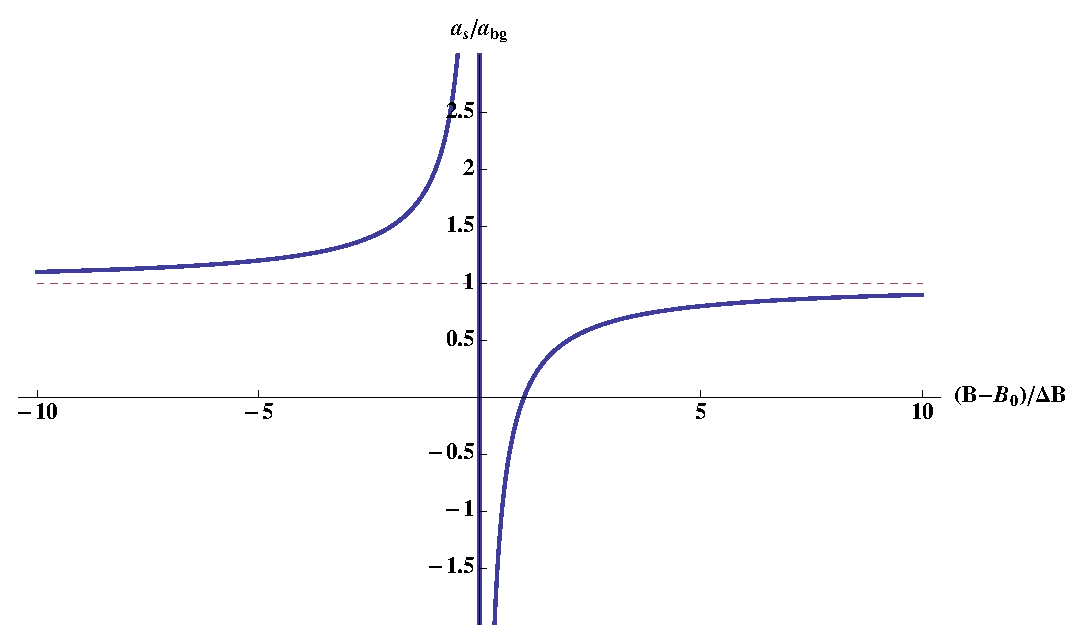
\includegraphics[width=0.8\textwidth]{FeshbachAs}
\caption{S-wave scattering length in Feshbach resonance} 
\label{fig:intro:Feshbach}
{\small Dashed line is $a_{bg}$.}
\end{center}
\end{figure}

Next we consider the bound state \footnote{Here we want to stress the difference between a closed-channel bound-state $\phi_{i}$ and a real bound state with negative energy formed by two channels.   The closed-channel bound state, $\phi_{i}$, is the eigenstate of the  isolated closed-channel Hamiltonian, and is not a real eigenstate for the full two-channel Hamiltonian.  On the other hand, the full  Hamiltonian has bound eigenstates ($E<0$) at large negative detuning (in the two-body context) or BEC-side (in the many-body context).  The bound state solution for a two-channel eigenstate has components both in the open-channel and the closed-channel.  Often the open-channel weight is larger when close to resonance and therefore those bound-states are often called open-channel bound-states.  Only at large negative detuning, the real two-channel bound state is mostly composed of close-channel component, and coincides with close-channel bound-state, $\phi_{i}$ to a large degree.}
where $E<0$, define
\begin{equation}\label{eq:intro:ab}
a_{b}(E)\equiv\frac{\hbar}{(2m_{r}\abs{E})^{1/2}}
\end{equation}
 Here we only study the bound state close to threshold with binding energy much smaller than the binding energy of closed-channel bound state $\phi_{0}$, $\abs{E}\ll{}E_{b}$, and therefore $a_{b}\gg{a_{c}}$.  Outside the range of potential $r_{c}$,  the wave function is proportional to $e^{-r/a_{b}}$. For $r_{c}\ll{}r\ll{}a_{b}$, it can be expanded as  $1-\frac{r}{a_{b}}$, just as the Bethe-Peierls boundary condition (or the s-wave scattering wave function) we discussed in Chapter \ref{sec:intro:as}.  Note that $a_{b}(E)$ is not identified as $a_{s}$ a priori.  We can go through the similar procedure as previous, and it is not hard to find
\begin{equation}
\frac{a_{bg}}{a_{b}}-1=\frac{-\mathcal{K}}{\delta+\mathcal{K}-E}
\end{equation}
Here we assume the short-range part of wave function $\chi$ does not change much and therefore $\mathcal{K}$ stays relatively constant.  Provided both $\delta$ and $\abs{E}$ are much smaller than $\mathcal{K}$, this leads to 
\begin{equation}\label{eq:intro:abKE}
a_{b}=\frac{\mathcal{K}}{\delta-E}
\end{equation}
It is not hard to see that $a_{b}$ indeed \emph{does} coincide with the s-wave scattering length $a_{s}$ when $\abs{E}\ll\abs{\delta}$, and therefore we will use them interchangeably hereafter. This is actually an example our discussion about the Bethe-Peierls boundary condition in Chapter \ref{sec:intro:as}.  Using Eqs. \ref{eq:intro:ab} and \ref{eq:intro:abKE}, it is easy to obtain an equation for $E$
\begin{equation}
(\abs{E}+\delta)^{2}-2\delta_{c}\abs{E}=0
\end{equation}
where $\delta_{c}$ is defined as 
\begin{equation}\label{eq:intro:deltaC}
\delta_{c}\equiv\frac{\mathcal{K}^{2}}{\hbar^{2}/m_{r}a_{bg}^{2}}
\end{equation}
And the solution is  (for $\delta<0$)
\begin{equation}
\abs{E}=\delta_{c}-\delta-\sqrt{\delta_{c}^{2}-2\delta\delta_{c}}
\end{equation}
Furthermore, we can calculate the ``relative weight'' (probability) of closed-channel 
\begin{equation}
\lambda=\br{\frac{1}{E-\tilde\delta}}^{2}\abs{\int{}dr'\phi_{0}(r')Y(r')\chi_{n}(r')}^{2}
\end{equation}
where $\chi_{n}(r)$ is the normalized open-channel bound-state component.  Comparing this with Eq. \ref{eq:intro:kappa}, assuming the short-range part of $\chi_{n}(r)$ does not differ from $\chi_{o}(r)$ much, we can find 
\begin{equation}
\lambda=\nth{(E-\tilde\delta)^{2}}\frac{\hbar^{2}}{2m_{r}a_{bg}}\mathcal{K}a_{b}^{-1}
\end{equation}
For $\abs{\delta}\lesssim\delta_{c}\ll\mathcal{K}$, $E-\tilde\delta\approx\mathcal{K}$ and we have 
\begin{equation}
\lambda=\frac{\hbar^{2}}{2m_{r}a_{bg}}\nth{(\mathcal{K}a_{b})}=\br{\frac{\abs{E}}{2\delta_{c}}}^{1/2}
\end{equation}
Now we can see that  $\delta_{c}$ is a ``characteristic'' energy scale. When $\abs{\delta}\gg\delta_{c}$, $E\approx\delta$, this simply means that when the negative detuning is large, most weight is in the closed-channel, and the real mixed bound state is a closed-channel bound state ($\phi_{0}$) dressed with little open-channel component and therefore the binding energy is roughly equal that of $\phi_{0}$.  The often quoted relation between $a_{s}$ and the binding energy (Eq. \ref{eq:intro:ab}) does not apply here.  On the contrary, when $\abs{\delta}\ll\delta_{c}$, $\abs{E}\approx-\delta^{2}/\delta_{c}\ll\delta$,  and closed-channel weight is much smaller than that of the open-channel, the real bound-state is more or less an open-channel affair with little dress-up from closed-channel.  % It is not hard to  estimate $\delta_{c}$. 

In many-body physics, another important energy scale comes into play, the Fermi energy, $E_{F}$.  When it is much smaller than $\delta_{c}$, i.e. a \emph{broad resonance},  closed-channel has only negligible weight close to resonance, where we are mostly interested in. In such situation, it is a good approximation to take the Feshbach resonance as only a knob to tweak the interaction in the open-channel.  On the contrary, when $E_{F}$ is close even larger than $\delta_{c}$, i.e. a \emph{narrow resonance}, the closed-channel weight can be  significant around resonance, therefore it is required to explicitly take the closed-channel into many-body framework.  










\chapter{The single-channel BEC-BCS crossover\label{sec:intro:1channel}}
In this chapter, we briefly review the BEC-BCS crossover in a single channel.   The idea to describe the BEC and BCS in the same footing stems back several decades \cite{Eagle, LeggettCrossover, Nozieres, RanderiaBEC}.  %One way to interpret BCS is through the existing macroscopic eigenvalue of two-body density matrix (see Sec. \ref{sec:intro:as})\cite{Leggett}.   This eigenvalue corresponds the more familiar anomalous expectation, $\av{a_{\uparrow-\vk}a_{\downarrow\vk}}$.  If simply taking it as wave function of a two-fermion molecule, this eigenfucntion, $\ket{\psi}=(\sum_{\vk}c_{\vk}a^{\dg}_{\uparrow\vk}a^{\dg}_{\downarrow-\vk})\ket{0}$ is very large in size (coherent length), much larger than the average particle distance.  Therefore overlap between different ``molecules'' is significant.   
The BCS theory can be understood as fermions form  ``giant molecules'' and those molecules then condense simultaneously.    It is not hard to show that the famous BCS ansatz is equivalent to  the  coherent state of a two-body pair $\psi^{\dg}=\sum_{\vk}c_{\vk}a^{\dg}_{\uparrow\vk}a^{\dg}_{\downarrow-\vk}$
\begin{equation}\label{eq:intro:BCScoherent}
\prod_{\vk}(u_{vk}+v_{\vk}a^{\dg}_{\uparrow\vk}a^{\dg}_{\downarrow-\vk})\ket{0}=A\exp{}(\sum_{\vk}c_{\vk}a^{\dg}_{\uparrow\vk}a^{\dg}_{\downarrow-\vk})\ket{0}
\end{equation}
where $c_{\vk}=( v_{\vk}/u_{\vk})$. The size of these ``giant molecules'' is in the order of coherent length and much larger than the interparticle distance.
Moving away from the BCS ends, a pair shrinks as the interparticle attraction becomes stronger.  At the BEC side, two-fermion molecules are smaller than the interparticle distance and therefore well-defined. However, the binding energy now is much higher than the typical many-body energy scale and condensation does not happens at the same time when molecules form.  Nevertheless,  at low enough temperature, we can still consider the formation of molecules and their condensation  at the same time, within the same framework as in BCS.  

In the single-channel BEC-BCS crossover model, one images a ``magic'' knob that can tunes the interaction strength along the crossover.  The many-body fermion  system sweeps from fermionic BCS to BEC of diatomic molecules  in response to the interaction change.   This applies directly to the broad-resonance of the two-channel case as well, where the closed-channel weight is negligible and serves only to modify the effective interaction strength in the open-channel.  We mostly follow the path-integral treatment in \cite{RanderiaBEC, Randeria1997, Randeria2008} because it can be readily adapted for two-channel model in the next chapter.
%\subsection{Path integral for one channels}
% !TeX root =thesis.tex
%\subsection{Path integral approach for single channel\label{sec:pathInt}}
\label{sec:pathInt}
Randeria and the company has studied this problem with path integral and it is proved to be a rather nice tool for the problem due to its flexibility and readiness for extension to higher order fluctuation.  

We start with an attractive $\delta$-potential in real space.  This is not equivalent to the l reduced pairing potential as in original BCS work.  However, reduced paring potential only couples  particles of the opposite momentum and does not support simple form of Hubbard-Stratonovich transformation, which is essential to solve the problem in path integral formulation.  
\begin{equation}
\hat{H}-\mu\hat{N}=\sum_{\sigma}\int{d^{d}r}c^{\dagger}_{\sigma}(\vr)\br{-\nth{2m}\nabla^{2}-\mu}c^{}_{\sigma}(\vr)-g\int{d^{d}r}c^{\dagger}_{\uparrow}(\vr)c^{\dagger}_{\downarrow}(\vr)c^{}_{\downarrow}(\vr)c^{}_{\uparrow}(\vr)
\end{equation}
 We can write down the action for the quantum partition function $\mathcal{Z}=\int{D(\bar\psi,\psi)\exp\br{-S[\bar\psi,\psi]}}$
\begin{equation}
S[\bar\psi,\psi]=\int^{\beta}_{0}d\tau\int{d^{d}r}\mbr{\sum_{\sigma}\bar\psi_{\sigma}(\vr,\tau)\br{\partial_{\tau}-\nth{2m}\nabla^{2}-\mu}\psi_{\sigma}(\vr,\tau)-g\bar\psi_{\uparrow}(\vr,\tau)\bar\psi_{\downarrow}(\vr,\tau)\psi^{}_{\downarrow}(\vr,\tau)\psi^{}_{\uparrow}(\vr,\tau)}
\end{equation}
We try to solve this system by introduce Hubbard-Stratonovich transformation.   Introduce a bosonic field $\Delta(\vr,\tau)$ coupled with Cooper channel $\psi(\vr,\tau)\psi(\vr,\tau)$. %Here we follow the normal notation from path integral, $r$ is four tempo-space coordinator.  
We write down first the Gaussian integral of $\Delta$
\begin{equation}
1=\int{D(\bar\Delta,\Delta)}\exp\br{-\nth{g}\int{d\tau{d}^{d}r}\bar\Delta\Delta}
\end{equation}
Note that we absorb the extra constant of integration into the measure of $D(\bar\Delta,\Delta)$.
And with a shift of $\Delta(\vr,\tau)\rightarrow\Delta(\vr,\tau)-g\psi(\vr,\tau)\psi(\vr,\tau)$, we have 
\footnote{$\int{D(\bar\Delta,\Delta)}\cdot1$ is only a constant factor on partition function $\mathcal{Z}$ and has no effect on real physical quantity, therefore, we can take it as 1, (equivalently divide the $\mathcal{Z}$ by a constant)}
\begin{equation}
\exp\br{g\int{d\tau{}d^{d}r}\psi_{\uparrow}\bar\psi_{\downarrow}\psi_{\downarrow}\psi_{\uparrow}}=
\int{D(\bar\Delta,\Delta)}\exp\bbr{-\int{d\tau{d^{d}r}}\mbr{\nth{g}\abs{\Delta}^{2}-\br{\bar\Delta\psi_{\downarrow}\psi_{\uparrow}+\Delta\bar\psi_{\uparrow}\bar\psi_{\downarrow}}}}
\end{equation}
Now the interaction term can be replaced.
\begin{equation*}
\mathcal{Z}=\int{D(\bar\psi,\psi)\int{D(\bar\Delta,\Delta)}\exp\bbr{-\int{d\tau{d^{d}r}}\mbr{\sum_{\sigma}\bar\psi_{\sigma}\br{\partial_{\tau}-\nth{2m}\nabla^{2}-\mu}\psi_{\sigma}+\nth{g}\abs{\Delta}^{2}-\br{\bar\Delta\psi_{\downarrow}\psi_{\uparrow}+\Delta\bar\psi_{\uparrow}\bar\psi_{\downarrow}}}}}
\end{equation*}
This form is bilinear to $\psi$, and we can rewrite it into a nicer form in Nambu spinor representation
\begin{equation}
\bar\Psi=\begin{pmatrix}\bar{\psi}_{\uparrow}&\psi_{\downarrow}\end{pmatrix}\text{,  }\qquad
\Psi=\begin{pmatrix}{\psi}_{\uparrow}\\\bar\psi_{\downarrow}\end{pmatrix}
\end{equation}
\begin{equation}
\mathcal{Z}=\int{D(\bar\psi,\psi)}\int{D(\bar\Delta,\Delta)}\exp
	\bbr{-\int{d\tau{d^{d}r}}\mbr{\nth{g}\abs{\Delta}^{2}-\bar\Psi \nG\Psi}}
\end{equation}
where 
\begin{equation}\label{eq:pathInt:nG}
\nG=\begin{pmatrix}
[\hat{G}_{0}^{(p)}]^{-1}&\Delta\\\bar\Delta&[\hat{G}_{0}^{(h)}]^{-1}
\end{pmatrix}
\end{equation}
is known as Gor'kov Green function, and $[\hat{G}_{0}^{(p)}]^{-1}=-\partial_{\tau}+\nth{2m}\nabla^{2}+\mu$, and $[\hat{G}_{0}^{(h)}]^{-1}=-\partial_{\tau}-\nth{2m}\nabla^{2}-\mu$ represent the non-interacting Green functions of the particle and hole respectively. Now $\Psi$ can be integrated out formally and partition function then only depends on bosonic field $\Delta$.
\begin{equation}\label{eq:pathInt:DeltaPF}
\mathcal{Z}=\int{D(\bar\Delta,\Delta)}\exp
	\bbr{-\mbr{\br{\int{d\tau{d^{d}r}}\nth{g}{\bar\Delta\Delta}}-\ln\det\nG}}
\end{equation}
And action is
\begin{equation}\label{eq:pathInt:DeltaAction}
S[\bar\Delta,\Delta]=
	{\mbr{\br{\int{d\tau{d^{d}r}}\nth{g}{\bar\Delta\Delta}}-\ln\det\nG}}
\end{equation}
Note that $\ln\det\nG$ goes through both the normal space and $2\times2$ Nambu spinor space.  

\subsection{Mean Field Result\label{sec:pathInt:meanfield}}
The saddle point equation of Eq. (\ref{eq:pathInt:DeltaPF}) gives the mean-field result of the system.  First we need to find the derivative of $\ln\det\nG$.  We notice the identity
\begin{equation}
\ln\det\hat{A}=\tr\ln\hat{A}
\end{equation}
and differential rule of a function like $\tr\ln$
\begin{equation}\label{eq:pathInt:diffTr}
\frac{\delta}{\delta\phi_q}\tr\ln(\nG)=\tr(\hat{\mathcal{G}}\frac{\delta}{\delta\phi_q}\nG)
\end{equation}
The saddle equation of Eq. (\ref{eq:pathInt:DeltaPF}) (differential with respect to $\Delta$) is
\begin{equation}
\nth{g}\bar{\Delta}(\vr,\tau)-\tr\mbr{\hat{\mathcal{G}}(\vr,\tau,\vr,\tau)\begin{pmatrix}0&1\\0&0\end{pmatrix}}=0
\end{equation}
Here this matrix is in the Nambu Spinor space.  If we seek a tempo-spacial homogeneous solution of $\Delta_0$, we can find the Nambu Green function from Eq. (\ref{eq:pathInt:nG}) in momentum space
\begin{equation}\label{eq:pathInt:G0}
G_0(p)=\nth{(i\omega_n)^2-E_\vp^2}
\begin{pmatrix}
	i\omega_n+\xi_\vp&-\Delta_0\\
	-\bar{\Delta}_0&i\omega_n-\xi_\vp
\end{pmatrix}
\end{equation}
Here $\omega_n$ is Matsubara frequency of Fermions.  $\xi_{\vk}=\epsilon_{\vk}-\mu$, $\epsilon_{\vk}=\vk^{2}/2m$,  $E_\vp=\sqrt{\xi_\vp^2+\abs{\Delta_0}^2}$.  And the saddle point equation can be rewritten as 
\begin{equation}
\nth{g}\bar{\Delta}_0=\frac{T}{L^d}\sum_{\vp,n}\frac{\bar\Delta_0}{\omega_n^2+E_\vp^2}
\end{equation}
The summation of Matsubara frequency can be evaluated and we find 
\begin{equation}
\nth{g}=\nth{L^d}\sum_{\vp}\frac{1-2n_f(E_p)}{2E_p}=\nth{L^d}\sum_{\vp}\frac{\tanh{(E_p/2T)}}{2E_p}
\label{eq:pathInt:gap}
\end{equation}
where $n_f(\epsilon)$ is the fermi distribution function.  This is exactly the gap equation obtained from other methods as well.  On the other hand, $\nG$ in Eq. (\ref{eq:pathInt:nG})  is the inverse of fermion-fermion correlation of $\Psi$.  In mean field, $G_{0}$ as Eq. (\ref{eq:pathInt:G0}) can be diagnosed in momentum space with a canonical (Bogoliubov) transformation.  Nevertheless, poles is where  $\omega^2-E_\vp^2=0$ (with a analytic continue of $i\omega_{n}\rightarrow\omega+0^{+}$) as we can see from  Eq. (\ref{eq:pathInt:G0}) and therefore the spectrum of fermionic excitation is $\pm{}E_{p}$.  

Summand in Eq. \ref{eq:pathInt:gap} does not decreases fast enough in 3D and the summation does not converges.  This is because our assumption of contact interaction breaks down when reaching real potential range $a_{c}$, i.e., the summation of momentum is capped at some high momentum $\Lambda$ related to $1/a_{c}$.  Notice that in 3-D, we have a relation that connect the bare potential $g$ to more physically observable s-wave scattering length $a_{s}$
\begin{equation}\label{eq:pathInt:as}
\frac{m}{4\pi{}a_{s}}=-\nth{g}+\sum_{k<\Lambda}\nth{2\epsilon_{\vk}}
\end{equation}
We can renormalize Eq. \ref{eq:pathInt:gap} with this relation
\begin{equation}
-\frac{m}{4\pi{}a_{s}}=\sum_{\vk}\mbr{\frac{\tanh{(E_k/2T)}}{2E_k}-\nth{2\epsilon_{\vk}}}
\end{equation}
Now the gap equation has proper decay in high momentum and no artificial cutoff is necessary.  There are two unknown parameters, $\mu$ and $\Delta$,  in the equation.  We need another equation in order to pin them down. To compliment the gap equation, we can introduce the number equation, $n=-\partial\Omega/\partial\mu$. At the saddle point, the thermodynamic potential is $\Omega_{0}=S[\Delta_{0}]/\beta$, and we have number equation
\begin{equation*}
n=-\nth{\beta}\tr\br{{G_{0}\pdiff{G_{0}^{-1}}{\mu}}}
\end{equation*}
similarly the summation over the Mastubara frequency can be evaluated and we have equation
\begin{equation}
n=\nth{L^{d}}\sum_{\vk}\mbr{1-\frac{\epsilon_{\vk}}{E_{\vk}}\tanh{(\frac{E_{\vk}}{2T})}}
\end{equation}

\subsection{Gaussian fluctuation and collective mode}\label{sec:collective1}
Once the mean field value is obtained, we can expand partition function Eq. (\ref{eq:pathInt:DeltaPF}) around it ($\Delta(\vr,\tau)=\Delta_{0}+\eta(\vr,\tau)$). The linear order of  expansion is zero because $\Delta_{0}$ is the saddle point.  The next order gives us the bilinear terms on $\eta$, i.e., correlation of bosonic field $\Delta$ (four-fermion correlation).  Note that here the hamiltonian only has an extreme-short-range ($\delta$) potential, therefore it cannot cover the situation of charged system where long-range Columnb interaction cannot be neglected.  We will discuss this later.  Nevertheless, it is conceivable that a more realistic short-range potential only renormalizes some parameters in the following calculation while leaves the qualitative result unmodified.  

Notice that we can expand the second term in Eq. \ref{eq:pathInt:DeltaPF} for $\hat{G}{}^{-1}=\hat{G}_{0}^{-1}+\hat{K}$
\begin{equation}\label{eq:pathInt:expand}
\tr\ln \hat{G}^{-1}=\tr\ln\hat{G_{0}}^{-1}+\tr(\hat{G_{0}}\hat{K})-\nth{2}\tr(\hat{G_{0}}\hat{K}\hat{G_{0}}\hat{K})+\cdots
\end{equation}
In our case,
\begin{equation}
\hat{K}=\begin{pmatrix}
0&\eta\\
\eta^{*}&0
\end{pmatrix}
\end{equation}
Here the linear terms of $\hat{K}$ or $\eta$ ($\eta^{*}$) are zero as the saddle point condition.  So to the second order, the action is 
\begin{equation}\label{eq:pathInt:DeltaActionGaussian}
S[\Delta_{0},\eta,\eta^{*}]=S[\Delta_{0}]+
	\nth{2g}\tr(\hat{K}\hat{K})+\nth{2}\tr(\hat{G_{0}}\hat{K}\hat{G_{0}}\hat{K})
\end{equation}
Write the last term into the momentum representation
\begin{equation}
\tr(\hat{G_{0}}\hat{K}\hat{G_{0}}\hat{K})=\sum_{q,p}\Tr\br{G_{0}({p})K_{q}G_{0}{}({p-q})K_{-q}}
\end{equation}
Notice that the second ``$\Tr$'' and following ``$\Tr$'' in this section only runs in Nambu spinor space and $q={(\vq,q_{l})}$, $p=(\vp,p_{n})$ are all four momentum, where $q_{l}$ is bosonic Matsubara frequency while $p_{n}$ is fermionic Matsubara frequency.
\begin{equation}
K_{q}=\begin{pmatrix}
0&\eta_{q}\\
\eta^{*}_{-q}&0
\end{pmatrix}
\end{equation}
If we introduce the a new vector 
\begin{equation}
\eta{(q)}=\begin{pmatrix}\eta_{q}\\\eta^{*}_{-q}\end{pmatrix}\qquad
\eta^{\dg}{(q)}=\begin{pmatrix}\eta^{*}_{q}&\eta_{-q}\end{pmatrix}
\end{equation}
the action can be rewritten into a more compact form
\begin{equation}
S[\Delta_{0},\eta,\eta^{*}]=S[\Delta_{0}]+\nth{2}\sum_{q}\Tr\mbr{\eta^{\dg}(q)\mathbf{M(q)}\eta(q)}
\end{equation}
Notice that we can always choose a real $\Delta_{0}$ and therefore $G_{0}{\ _{12}}(p)=G_{0}{\ _{21}}(p)$, we have 
\begin{equation}
\mathbf{M(q)}=
\begin{pmatrix}
\nth{g}+\sum_{p}G_{0}{\ }_{11}(p)G_{0}{\ }_{22}(p-q)&\sum_{p}G_{0}{\ }_{12}(p)G_{0}{\ }_{12}(p-q)\\
\sum_{p}G_{0}{\ }_{12}(p)G_{0}{\ }_{12}(p-q)&\nth{g}+\sum_{p}G_{0}{\ }_{11}(p-q)G_{0}{\ }_{22}(p)
\end{pmatrix}
\end{equation}
The summation over (fermionic) Matsubara frequency of $p_{n}$ can be carried out at zero temperature
\footnote{\label{foot:intro:sum}The summation of Matsubara frequency of function $h(i\omega_{n})$ is carried out by the normal method to multiplying $h(z)$ with fermi distribution function $n_{F}(z)$, and then find all residues with a contour over infinity.  However, due to zero temperature, the  $n_{F}(z)$ only nonzero at the negative singular points of $h(z)$, $-E_{\vk}$ in our case.  (The other singular point $E_{\vk}$ gives $n_{F}(E_{\vk})=0$ for zero temperature.}
\begin{equation}
\begin{split}
M_{11}(q)&=M_{22}(-q)\\
	&=\nth{g}+\sum_{\vp{,}p_{n}}G_{0}{\ }_{11}(p)G_{0}{\ }_{22}(p-q)\\
	&=\nth{g}+\sum_{\vp}\br{\frac{u^{2}u'^{2}}{iq_{l}-E-E'}-\frac{v^{2}v'^{2}}{iq_{l}+E+E'}}
\end{split}
\end{equation}
\begin{equation}
\begin{split}
M_{12}(q)&=M_{21}(q)\\
	&=\sum_{\vp{,}p_{n}}G_{0}{\ }_{12}(p)G_{0}{\ }_{12}(p-q)\\
	&=\sum_{\vp}uvu'v'\br{\nth{iq_{l}+E+E'}-\nth{iq_{l}-E-E'}}
\end{split}
\end{equation}
where $u=u_{\vp}$, $v=v_{\vp}$, $E=E_{\vp}$ and $u'=u_{\vp-\vq}$, $v'=v_{\vk-\vq}$, $E'=E_{\vk-\vq}$.  $u$, $v$, $E$ are as defined usually in BCS literature. 
\begin{equation}
v_{\vk}^{2}=1-u_{\vk}^{2}=\nth{2}\br{1-\frac{\xi_{\vk}}{E_{\vk}}}
\end{equation}
 The $G^{(M)}=\mathbf{M}^{-1}$ is the correlation function of $\eta$ (or $\Delta$) and its poles give the spectrum of collective mode as every  $\eta_{q}$ (or $\Delta_{q}$) involves many fermions moving in a coherent manner.  So the spectrum of collective modes can be determined by $\det{M(\omega,\vq)}=0$ after we analytically continue for the frequency $iq_{l}\rightarrow\omega+i0^{+}$.  
 
For low energy modes, where $\omega,\,\abs{\vq}^{2}\ll\min\bbr{E_{\vk}}$ both are much smaller than $\Delta_{0}$, we can expand $M$ with $\omega$ and $\vq$.  


\subsection{Alternative in inverting green function\label{sec:diagonalizeGreen1}}
In the above section, we have inversion of Gorkov green function Eq. (\ref{eq:pathInt:nG}) and it can be invert easily as Eq. (\ref{eq:pathInt:G0}).   Alternatively, we can use a different approach which proves to be more convenient in two-channel problem.  First, we diagonalize $\nG$ with unitary transformation $T$, in momentum space
\begin{equation}
\nG=\mtrx{i\omega_{n}-\xi_{k}&\Delta\\\bar\Delta&i\omega_{n}+\xi_{k}}=T^{\dg}BT
\end{equation}
It is easy to show that such $T$ and $B$ satisfing above equation are
\begin{equation}
T=\mtrx{u_{k}&v_{k}\\-v_{k}^{*}&u_{k}}\qquad{}B=\mtrx{i\omega_{n}+E_{k}&0\\0&i\omega_{n}-E_{k}}
\end{equation}
where $u_{k}^{2}(v_{k}^{2})=\nth{2}(1\pm\xi_{k}/E_{k})$ and $E_{k}$ are conventionally defined quantities in BCS theory.   Actually, this transformation is nothing but Bogoliubov canonical transformation, and $B$ matrix simply describes spectrum of fermionic quasi-particles.  Now it is easy to invert $\nG$
\begin{equation}
G=T^{\dg}B^{-1}T
\end{equation}
Green's function $G$ takes a more conventional form $A/(i\omega_{n}-e_{k})$ without any dependency on frequency in nominator as Eq. (\ref{eq:pathInt:G0}). Matsubara frequency summation over $G_{0}(k)$ in mean-field and $G_{0}(k)G_{0}(k+q)$ in Gaussian order are then fairly straight-forward as in text-book.  




\begin{subappendices}
\end{subappendices}

